\documentclass[conference]{IEEEtran}
\IEEEoverridecommandlockouts
% The preceding line is only needed to identify funding in the first footnote. If that is unneeded, please comment it out.
\usepackage{cite}
\usepackage{amsmath,amssymb,amsfonts}
\usepackage{algorithmic}
\usepackage{graphicx}
\usepackage{textcomp}
\usepackage{xcolor}
\def\BibTeX{{\rm B\kern-.05em{\sc i\kern-.025em b}\kern-.08em
    T\kern-.1667em\lower.7ex\hbox{E}\kern-.125emX}}
\begin{document}

%LDP机制下的快速FIM方法-    标题
\title{Fast top-k frequent itemset mining under Local Differential Privacy*\\
{\footnotesize \textsuperscript{*}Note: Sub-titles are not captured in Xplore and
should not be used}
\thanks{Identify applicable funding agency here. If none, delete this.}
}

\author{\IEEEauthorblockN{1\textsuperscript{st} Wang JiaLi}
\IEEEauthorblockA{\textit{dept. name of organization (of Aff.)} \\
\textit{name of organization (of Aff.)}\\
City, Country \\
email address or ORCID}
%\and
%\IEEEauthorblockN{2\textsuperscript{nd} Given Name Surname}
%\IEEEauthorblockA{\textit{dept. name of organization (of Aff.)} \\
%\textit{name of organization (of Aff.)}\\
%City, Country \\
%email address or ORCID}
%\and
%\IEEEauthorblockN{3\textsuperscript{rd} Given Name Surname}
%\IEEEauthorblockA{\textit{dept. name of organization (of Aff.)} \\
%\textit{name of organization (of Aff.)}\\
%City, Country \\
%email address or ORCID}
%\and
%\IEEEauthorblockN{4\textsuperscript{th} Given Name Surname}
%\IEEEauthorblockA{\textit{dept. name of organization (of Aff.)} \\
%\textit{name of organization (of Aff.)}\\
%City, Country \\
%email address or ORCID}
%\and
%\IEEEauthorblockN{5\textsuperscript{th} Given Name Surname}
%\IEEEauthorblockA{\textit{dept. name of organization (of Aff.)} \\
%\textit{name of organization (of Aff.)}\\
%City, Country \\
%email address or ORCID}
%\and
%\IEEEauthorblockN{6\textsuperscript{th} Given Name Surname}
%\IEEEauthorblockA{\textit{dept. name of organization (of Aff.)} \\
%\textit{name of organization (of Aff.)}\\
%City, Country \\
%email address or ORCID}
}

\maketitle

\begin{abstract}
This is the abstract.
\end{abstract}

\begin{IEEEkeywords}
This is the keywords
\end{IEEEkeywords}

\section{Introduction}
%2020年2月26日,差分隐私技术被全球知名科技评论期刊《麻省理工学院技术评论》评为“全球十大突破性技术”。差分隐私是密码学中的一种手段,旨在提供一种当从统计数据库查询时,最大化数据查询的准确性,同时最大限度减少识别其记录的机会。作为一种数学技术,它能够在给数据添加噪声的同时,量化计算隐私提升的程度,从而使得增加“噪音”的过程变得更加严谨。
Differential privacy (DP)\cite{a7} is the state-of-the-art approach that is used to protect individual privacy in the process of data collection, which has been named one of the world's top 10 breakthrough technologies in 2020 by the MIT technology review. It is a means in cryptography that aims to provide a way to maximize the accuracy of data queries when querying from statistical databases while minimizing the chances of identifying their records. Meanwhile, as a mathematical technique, it can add noise to the data while quantifying the extent of the increase in privacy, thus making the process of adding ``noise'' more rigorous.

%差分隐私技术因其独特的优势,被学术界及工业界广泛的研究。谷歌、微软、苹果等公司使用该技术在保护用户隐私的同时,手机聚合数据,从而提升服务质量。并且美国政府将要完成2020年对3.3亿美国居民的人口普查,同时还要对他们的身份数据进行保密。如果任务完成顺利,这将是迄今为止规模最大的应用。
Due to its unique advantages, DP has been widely studied by the academia and industry. For example, Google, Microsoft, apple and other companies use this technology to protect users' privacy, and at the same time, mobile phones aggregate data, so as to improve service quality. And the U.S. government is to complete a census of 330 million U.S. residents by 2020, keeping their identities secret, in what would be the largest application of DP ever.

%差分隐私可分为CDP和LDP。相对于CDP,LDP不需要可信第三方的假设条件并且提供了更强的隐私保证。LDP的研究涉及很多方面,近年来,在数据挖掘方面的工作引起了人们的关注。  简单介绍以下CDP的DM工作。
There are two types of differential privacy - Centralized differential privacy (CDP) and Local differential privacy (LDP). Compared with CDP, the LDP does not require the assumptions of a trusted third party and provides stronger privacy guarantees.  {\color{red}DP's research has involved many aspects, in recent years, the work in mining frequent itemsets has attracted the attention, which is one of  the most important techniques because of its ability to locate the repeating relationships between different items in a data set and plays an essential role in mining association rules\cite{apriori}. Formally, let $I = \{x_1,x_2,...,x_d\}$ be a set of items and $D = <T_1,T_2,...,T_n>$ denote a transaction database, where $T_i(i \in [1...n])$ is a transaction that is a subset of $I$. A sample of transational data is shown in Table \ref{trans table}. The support of an itemset $X$, where $X \subset I$ is a set of items, is the number of transactions containing $X$ in $D$. Given a minimum support threshold $\delta$, the problem of finding the complete set of frequent itemsets that supports no less than $\delta$ is called the frequent itemset mining (FIM) problem.}

\begin{table}[htbp]
\caption{{\color{red}Sample of transactional data.}}
\begin{center}
\begin{tabular}{|c|l|}\hline
  TID&List of items \\\hline
  T01&$a,f,c,g,p$ \\\hline
  T02&$a,b,c,f,l,o$ \\\hline
  T03&$b,f,h,o$ \\\hline
  T04&$b,c,p$ \\\hline
  T05&$f,a,c,l,p,n$ \\\hline
\end{tabular}
\label{trans table}
\end{center}
\end{table}

%CDP的FIM简单介绍
A lot of work\cite{a3,a4,a5,a6} has been done to solve DM problems in CDP. However, since the analyst holds the user's raw data in CDP setting, its main job is to add noise to the results to satisfy the DP definition.

%在本文中,我们考虑交易数据集下的FIM问题
In this paper, we consider the $top-k$ FIM problem in transaction databases under LDP setting.However, there is no reliance on third party assumptions in LDP. The data analyst wants to find $k$ itemsets with highest support while while users are sensitive and unwilling to answer their real infomation. The main challenge is that the analyst does not hold the user's original sensitive information, which makes it quite difficult to mine useful information with sanitized data. Qin et al.\cite{a1} point out that if utlize directly existing FIM algorithm (e.g. Apriori\cite{apriori,apr}, FP-growth\cite{fp}, Eclat\cite{eclat}) would result in accumulation of dramatic noise because of multi-iteration between users and analyst.

%引出LDP下的DM方法,然后给出SVSM的具体细节,并指出本文工作解决重点。
Specifically for FIM in the local setting, Qin et al.\cite{a1} leave it as a future work but there is no clear solution. Wang et al.\cite{a2} solves  the $top-k$ frequent itemset mining (FIM) task for the first time with \textbf{padding-and-sampling-based frequency oracle} (PSFO). In \cite{a2}, the Set-Value Item Mining (SVIM) protocol has been proposed to handles set values under the LDP setting, with the purpose of finding the $k$ most frequent items and their frequencies. To mine frequent itemsets , a core technique is {\color{red}``Guessing Frequency (GF)''}. That is, the analyst first calculated  the frequency of a given itemset $X$ for all candidate itemsets by \eqref{gf},
\begin{equation}
\varphi(X)=\prod_{x \in X} \mu(x) , \mu(x) = \frac{0.9\times \tilde{\theta}(x)}{\max \limits_{x \in S^{\prime}} \tilde{\theta}(x)}\label{gf}
\end{equation}
where $\varphi(X)$ represents the speculative frequency of itemset $X$, $S^{\prime}$ and $\tilde{\theta}(x)$ are denoted separately the $top-k$ frequent items set and the frequency of a given item $x$. Then $2k$ itemsets with highest guessing frequencies are selected to construct candidate set $IS$. Finally, reference \cite{a2} utilized SVIM protocol again with the domain $IS$ to mine $top-k$ itemsets. We observe that, the size of candidate set to construct $IS$ increase significantly with $k$. As a result, it is computationally expensive when $k$ is large (e.g., $k=100$). 

%介绍本文工作_______________________之前需要介绍以下与FPtree的结合
Inspiringly, we propose {\color{red}minefp} protocol, which aims at finding $top-k$ itemsets under the LDP setting and provides similar accuracy while providing lower overhead than existing SVSM protocol within the same privacy constraints.
First, the SVIM protocol is used to estimate the $k$ most frequent items and their frequencies. Second, users report the number of frequent items they have; the analyst estimates the distribution user reported and figure out the right $M$ as the maximum iteration of the tree. Third, users interact with the analyst to build effectively the FP-tree\cite{fp}. Fourth, the analyst optimizes and mines the FP-tree. Fifth, the analyst publishes $top-k$ itemsets.Experimental results how that {\color{red}minefp
outperforms SVSM in that it identifies quickly frequent itemsets as well as estimates the frequencies more accurately.}

{\color{red}
To summarize, the main contributions of this paper are:
\begin{itemize}
\item We study the application of FP-growth algorithm and design the FP-tree-based-mine (minefp) protocol to find frequent itemsets as well as their frequencies in the LDP setting. Experimental results on real-world datasets show the significant improvement over previous techniques.
\item We investigate GF to construct candidate set and point out that it is beneficial to build hierarchically FP-tree. 
\end{itemize}
}


%SVSM的主要缺点然后引出本文方案
\textbf{Roadmap.}

\section{Background}
\subsection{Local Differential Privacy (LDP)}
In the local setting, there is no trusted third party and an aggregator wants to gather information from users, where each user possesses an input $v$. The privacy of the data contributor is protected by perturbing her/his original data at the data contributor’s side; thus, the agregator cannot access the original data, but is still able to obtain population statistics.

Formally, let $D$ denote the whole  transaction databases. $\epsilon$-local differential privacy (or $\epsilon$-LDP) is defined on an algorithm $\mathcal{A}$ and a privacy budget $\epsilon \geq 0$ as follows.

\newtheorem{Definition}{\bf Definition}
\begin{Definition}
($\epsilon-LDP$). A randomized algorithm $\mathcal{A}$ satisfies $\epsilon$-local differential privacy ($\epsilon$-LDP), if and only if for (1) all pairs of input $v_i,v_j \in D$, and (2) any possible output $\mathcal{O}$ of $\mathcal{A}$, we have:\\
$$\frac{\mathbf{Pr}[\mathcal{A}(v_i)=\mathcal{O}]}{\mathbf{Pr}[\mathcal{A}(v_j)=\mathcal{O}]} \leq e^{\epsilon}$$
\end{Definition}

$Sequential\  composability$\cite{a9} and $post-processing$\cite{post-processing} are vitally important properties of differential privacy. The former allows each user to divide privacy budget into multiple portions and use each portion to execute independent LDP protocols on the same input while the sequential executions provide $\sum \epsilon_i$-LDP; the latter guarantees that any processing of the noisy data do not disclose the privacy.

\newtheorem{theorem}{\bf Theorem}[section]
\begin{theorem}\label{sequential composability}
$(sequential\ composability)$. Given $m$ randomized algorithms $\mathcal{A}_i(1 \leq i \leq m)$, each of which satisfies $\epsilon_i$-local differential privacy. Then the sequence of $\mathcal{A}_i$ collectively provides $(\sum_{i=1}^{m} \epsilon_i)$-local differential privacy. 
\end{theorem}

\begin{theorem}\label{post processing}
$(post-processing)$. For any method $\phi$ which works on the output of a $\epsilon$-LDP algorithm $\mathcal{A}$ without accessing the raw data, the procedure $\phi \big(\mathcal{A(\cdot)} \big)$ remains $\epsilon$-LDP.
\end{theorem}


\subsection{LDP Protocols}
A frequency oracle (FO) protocol enables the estimation of the frequency of any given value $v \in D$ under LDP. Randomized response (RR)\cite{rr} is a traditional technique for estimating unbiasedly a population proprotion, which is the building block of many LDP protocols, such as RAPPOR\cite{rappor}, GRR and OLH\cite{a8}. Suppose the respondents were asked to answer a sensitive Boolean question (e.g. have you ever cheated on your partner?) in a survey and provisions made for each person to be interviewed. That is, each respondent gives the raw answer with probability $p$ and gives the opposite answer with probabilit $q = 1-p$. Specially, to satisfy $\epsilon$-LDP, the probability p is set to $\frac{e^{\epsilon}}{1+e^{\epsilon}}$. 

Then, the agregator calculates the estimated percentage of ``Yes'' (denote as $\tilde{\theta}$) as example  from all sanitized answers, which is unbiased, as follows: 
$$\tilde{\theta}(Yes) = \frac{\mathcal{C}(answer=Yes) - nq}{p-q}$$
where $n$ is the total number of respondents and $\mathcal{C}(answer=Yes)$ denotes the number of occurrences respondents answered ``Yes''. Accordingly, the variance of it is 
$$Var \big[\tilde{\theta}(Yes) \big] = $$

However, the RR protocol only applies to binary Boolean problems, which greatlt limits its application. Therefore, in \cite{a8}, two effective protocols, Generalized Random Response (GRR) and Optimized Local Hash (OLH), are proposed for the purpose of solving problems with large domain size $\mathcal{D}$. Specially, GRR extends the RR protocol by setting probability $p = \frac{e^{\epsilon}}{e^{\epsilon} + \mathcal{D} - 1}$ to give the raw answer $y = v$ and probability $q = \frac{1-p}{\mathcal{D}-1}$ (i.e. $q =\frac{1}{e^{\epsilon} + \mathcal{D} - 1}$) to give the perturbed answer $y \neq v$. It is shown that RR is the special case while $\mathcal{D} = 2$. 

In \cite{a8}, it turns out that when d is large, the OLH protocol provides the best accuracy while maintaining a low communication cost.  In this paper, we use the OLH protocol as a primitive and describe it below.

$Optimized\ Local\ Hashing\ (OLH)$\cite{a8}: In order to deal with a large domain size $\mathcal{D}$ as well as reduce the communication cost, OLH protocol applys a hash function to map each input value into a value in $[g]$, where $g \geq 2$ and $g \ll \mathcal{D}$. Then randomized response is used to the hashed value in the smaller domain. In \cite{a8}, the optimal choice of the parameter $g$ is $\lceil e^{\epsilon}+1 \rceil$ which meets the minimal variance.

Let $H$ is randomly chosen from a family of hash functions that outputs a value in $[g]$ and $x = H(v)$. The perturbing protocol in OLH is $Perturb \big(\langle H,x \rangle \big) = \langle H,y \rangle$, where
$$\forall_{i\in [g]} \mathbf{Pr} [y=i] = 
\begin{cases}
p = \frac{e^{\epsilon}}{e^{\epsilon}+g-1},&\text{if $x=i$} \\
q = \frac{1}{e^{\epsilon}+g-1},&\text{if $x\neq i$}
\end{cases}
$$

Accordingly, the aggregator first calculates the number of perturbed values that ``supports'' that the input is $v$ (denote as $\mathcal{C}(v)$), then transforms $\mathcal{C}(v)$ to its unbiased estimation
\begin{equation}
\tilde{\theta}(v) := \frac{\mathcal{C}(v) - n/g}{p-1/g}
\label{olh aggregate}
\end{equation}

The variance of this estimation is 
\begin{equation}
Var\big[\tilde{\theta}(v)\big] =n \cdot \frac{4e^{\epsilon}}{{(e^{\epsilon}-1)}^2}
\label{olh variance}
\end{equation}

In \cite{a8}, it suggests that when $\mathcal{D}<3e^{\epsilon} +2$, GRR is the best among all approaches; but for large domain size $\mathcal{D}$, OLH meets better performance and has a variance that does not depend on $\mathcal{D}$.

$------------$

%%%%%%
{\color{red}In \cite{a8}, the two best performing FO protocols are Generalized Random Response (GRR) and Optimized Local Hash (OLH). The former extends the randomized response (RR) technique\cite{rr}, which is an old technique developed for the interviewees in a survey to give random answer to a sensitive boolean question so that they can achieve plausible deniability; the latter deals with a large domain size $|I|$ by hashing a large domain size $|I|$ to a smaller size $g$ and applying RR to the hashed value. It was found that GRR offers the best accuracy than OLH when $|I| < 3e^{\epsilon} + 2$, where $|I|$ is the size of the domain of items under consideration. Therefore, in  \cite{a2}, an adaptive FO protocol can be proposed from the known $I$ as well as $\epsilon$.\\}
\textbf{Generalized Random Response (GRR)}

\subsection{FP-growth algorithm}
Frequent pattern growth (FP-growth)\cite{fp} is an algorithm that mines the complete set of frequent patterns without a costly candidate generation process, which based on the frequent pattern tree (FP-tree) structure that is an extended prefix-tree structure for storing compressed, crucial information about frequent patterns. The FP-Tree is further divided into a set of Conditional FP-Trees for each frequent item so that they can be mined separately. An example of the FP-Tree that represents the frequent items is shown in Fig. \ref{fptree}, where the minimum support threshold is set to 3.

%A sample of transational data is shown in Table \ref{trans table}.

The FP-growth algorithm solves the problem of identifying long frequent itemsets by searching through smaller conditional FP-tree repeatedly. The conditional pattern base is a “sub-database” which consists of every prefix path in the FP-Tree that co-occurs with every frequent length-1 item. It is used to construct the conditional FP-tree and generate all the frequent patterns related to every frequent length-1 item. In this way, the cost of searching for the frequent patterns is substantially reduced.

\begin{figure}[htbp]
\centerline{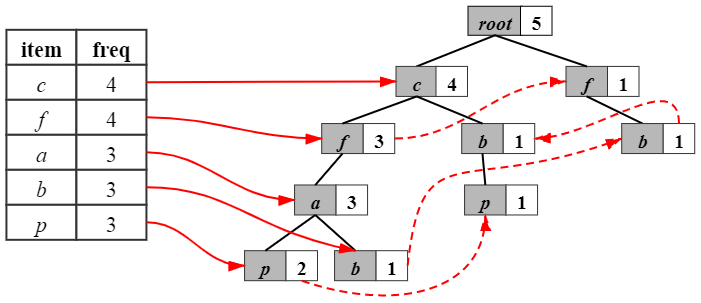
\includegraphics[width=0.45\textwidth]{fptree.png}}
\caption{Frequrnt pattern tree(FP-tree).}
\label{fptree}
\end{figure}

\section{Ease of Use}

\subsection{Maintaining the Integrity of the Specifications}

The IEEEtran class file is used to format your paper and style the text. All margins, 
column widths, line spaces, and text fonts are prescribed; please do not 
alter them. You may note peculiarities. For example, the head margin
measures proportionately more than is customary. This measurement 
and others are deliberate, using specifications that anticipate your paper 
as one part of the entire proceedings, and not as an independent document. 
Please do not revise any of the current designations.

\section{Prepare Your Paper Before Styling}
Before you begin to format your paper, first write and save the content as a 
separate text file. Complete all content and organizational editing before 
formatting. Please note sections \ref{AA}--\ref{SCM} below for more information on 
proofreading, spelling and grammar.

Keep your text and graphic files separate until after the text has been 
formatted and styled. Do not number text heads---{\LaTeX} will do that 
for you.

\subsection{Abbreviations and Acronyms}\label{AA}
Define abbreviations and acronyms the first time they are used in the text, 
even after they have been defined in the abstract. Abbreviations such as 
IEEE, SI, MKS, CGS, ac, dc, and rms do not have to be defined. Do not use 
abbreviations in the title or heads unless they are unavoidable.

\subsection{Units}
\begin{itemize}
\item Use either SI (MKS) or CGS as primary units. (SI units are encouraged.) English units may be used as secondary units (in parentheses). An exception would be the use of English units as identifiers in trade, such as ``3.5-inch disk drive''.
\item Avoid combining SI and CGS units, such as current in amperes and magnetic field in oersteds. This often leads to confusion because equations do not balance dimensionally. If you must use mixed units, clearly state the units for each quantity that you use in an equation.
\item Do not mix complete spellings and abbreviations of units: ``Wb/m\textsuperscript{2}'' or ``webers per square meter'', not ``webers/m\textsuperscript{2}''. Spell out units when they appear in text: ``. . . a few henries'', not ``. . . a few H''.
\item Use a zero before decimal points: ``0.25'', not ``.25''. Use ``cm\textsuperscript{3}'', not ``cc''.)
\end{itemize}

\subsection{Equations}
Number equations consecutively. To make your 
equations more compact, you may use the solidus (~/~), the exp function, or 
appropriate exponents. Italicize Roman symbols for quantities and variables, 
but not Greek symbols. Use a long dash rather than a hyphen for a minus 
sign. Punctuate equations with commas or periods when they are part of a 
sentence, as in:
\begin{equation}
a+b=\gamma\label{eq}
\end{equation}

Be sure that the 
symbols in your equation have been defined before or immediately following 
the equation. Use ``\eqref{eq}'', not ``Eq.~\eqref{eq}'' or ``equation \eqref{eq}'', except at 
the beginning of a sentence: ``Equation \eqref{eq} is . . .''

\subsection{\LaTeX-Specific Advice}

Please use ``soft'' (e.g., \verb|\eqref{Eq}|) cross references instead
of ``hard'' references (e.g., \verb|(1)|). That will make it possible
to combine sections, add equations, or change the order of figures or
citations without having to go through the file line by line.

Please don't use the \verb|{eqnarray}| equation environment. Use
\verb|{align}| or \verb|{IEEEeqnarray}| instead. The \verb|{eqnarray}|
environment leaves unsightly spaces around relation symbols.

Please note that the \verb|{subequations}| environment in {\LaTeX}
will increment the main equation counter even when there are no
equation numbers displayed. If you forget that, you might write an
article in which the equation numbers skip from (17) to (20), causing
the copy editors to wonder if you've discovered a new method of
counting.

{\BibTeX} does not work by magic. It doesn't get the bibliographic
data from thin air but from .bib files. If you use {\BibTeX} to produce a
bibliography you must send the .bib files. 

{\LaTeX} can't read your mind. If you assign the same label to a
subsubsection and a table, you might find that Table I has been cross
referenced as Table IV-B3. 

{\LaTeX} does not have precognitive abilities. If you put a
\verb|\label| command before the command that updates the counter it's
supposed to be using, the label will pick up the last counter to be
cross referenced instead. In particular, a \verb|\label| command
should not go before the caption of a figure or a table.

Do not use \verb|\nonumber| inside the \verb|{array}| environment. It
will not stop equation numbers inside \verb|{array}| (there won't be
any anyway) and it might stop a wanted equation number in the
surrounding equation.

\subsection{Some Common Mistakes}\label{SCM}
\begin{itemize}
\item The word ``data'' is plural, not singular.
\item The subscript for the permeability of vacuum $\mu_{0}$, and other common scientific constants, is zero with subscript formatting, not a lowercase letter ``o''.
\item In American English, commas, semicolons, periods, question and exclamation marks are located within quotation marks only when a complete thought or name is cited, such as a title or full quotation. When quotation marks are used, instead of a bold or italic typeface, to highlight a word or phrase, punctuation should appear outside of the quotation marks. A parenthetical phrase or statement at the end of a sentence is punctuated outside of the closing parenthesis (like this). (A parenthetical sentence is punctuated within the parentheses.)
\item A graph within a graph is an ``inset'', not an ``insert''. The word alternatively is preferred to the word ``alternately'' (unless you really mean something that alternates).
\item Do not use the word ``essentially'' to mean ``approximately'' or ``effectively''.
\item In your paper title, if the words ``that uses'' can accurately replace the word ``using'', capitalize the ``u''; if not, keep using lower-cased.
\item Be aware of the different meanings of the homophones ``affect'' and ``effect'', ``complement'' and ``compliment'', ``discreet'' and ``discrete'', ``principal'' and ``principle''.
\item Do not confuse ``imply'' and ``infer''.
\item The prefix ``non'' is not a word; it should be joined to the word it modifies, usually without a hyphen.
\item There is no period after the ``et'' in the Latin abbreviation ``et al.''.
\item The abbreviation ``i.e.'' means ``that is'', and the abbreviation ``e.g.'' means ``for example''.
\end{itemize}
An excellent style manual for science writers is \cite{b7}.

\subsection{Authors and Affiliations}
\textbf{The class file is designed for, but not limited to, six authors.} A 
minimum of one author is required for all conference articles. Author names 
should be listed starting from left to right and then moving down to the 
next line. This is the author sequence that will be used in future citations 
and by indexing services. Names should not be listed in columns nor group by 
affiliation. Please keep your affiliations as succinct as possible (for 
example, do not differentiate among departments of the same organization).

\subsection{Identify the Headings}
Headings, or heads, are organizational devices that guide the reader through 
your paper. There are two types: component heads and text heads.

Component heads identify the different components of your paper and are not 
topically subordinate to each other. Examples include Acknowledgments and 
References and, for these, the correct style to use is ``Heading 5''. Use 
``figure caption'' for your Figure captions, and ``table head'' for your 
table title. Run-in heads, such as ``Abstract'', will require you to apply a 
style (in this case, italic) in addition to the style provided by the drop 
down menu to differentiate the head from the text.

Text heads organize the topics on a relational, hierarchical basis. For 
example, the paper title is the primary text head because all subsequent 
material relates and elaborates on this one topic. If there are two or more 
sub-topics, the next level head (uppercase Roman numerals) should be used 
and, conversely, if there are not at least two sub-topics, then no subheads 
should be introduced.

\subsection{Figures and Tables}
\paragraph{Positioning Figures and Tables} Place figures and tables at the top and 
bottom of columns. Avoid placing them in the middle of columns. Large 
figures and tables may span across both columns. Figure captions should be 
below the figures; table heads should appear above the tables. Insert 
figures and tables after they are cited in the text. Use the abbreviation 
``Fig.~\ref{fig}'', even at the beginning of a sentence.

\begin{table}[htbp]
\caption{Table Type Styles}
\begin{center}
\begin{tabular}{|c|c|c|c|}
\hline
\textbf{Table}&\multicolumn{3}{|c|}{\textbf{Table Column Head}} \\
\cline{2-4} 
\textbf{Head} & \textbf{\textit{Table column subhead}}& \textbf{\textit{Subhead}}& \textbf{\textit{Subhead}} \\
\hline
copy& More table copy$^{\mathrm{a}}$& &  \\
\hline
\multicolumn{4}{l}{$^{\mathrm{a}}$Sample of a Table footnote.}
\end{tabular}
\label{tab1}
\end{center}
\end{table}

\begin{figure}[htbp]
\centerline{
\includegraphics{fig1.png}}
\caption{Example of a figure caption.}
\label{fig}
\end{figure}

Figure Labels: Use 8 point Times New Roman for Figure labels. Use words 
rather than symbols or abbreviations when writing Figure axis labels to 
avoid confusing the reader. As an example, write the quantity 
``Magnetization'', or ``Magnetization, M'', not just ``M''. If including 
units in the label, present them within parentheses. Do not label axes only 
with units. In the example, write ``Magnetization (A/m)'' or ``Magnetization 
\{A[m(1)]\}'', not just ``A/m''. Do not label axes with a ratio of 
quantities and units. For example, write ``Temperature (K)'', not 
``Temperature/K''.

\section*{Acknowledgment}

The preferred spelling of the word ``acknowledgment'' in America is without 
an ``e'' after the ``g''. Avoid the stilted expression ``one of us (R. B. 
G.) thanks $\ldots$''. Instead, try ``R. B. G. thanks$\ldots$''. Put sponsor 
acknowledgments in the unnumbered footnote on the first page.

\section*{References}

Please number citations consecutively within brackets \cite{b1}. The 
sentence punctuation follows the bracket \cite{b2}. Refer simply to the reference 
number, as in \cite{b3}---do not use ``Ref. \cite{b3}'' or ``reference \cite{b3}'' except at 
the beginning of a sentence: ``Reference \cite{b3} was the first $\ldots$''

Number footnotes separately in superscripts. Place the actual footnote at 
the bottom of the column in which it was cited. Do not put footnotes in the 
abstract or reference list. Use letters for table footnotes.

Unless there are six authors or more give all authors' names; do not use 
``et al.''. Papers that have not been published, even if they have been 
submitted for publication, should be cited as ``unpublished'' \cite{b4}. Papers 
that have been accepted for publication should be cited as ``in press'' \cite{b5}. 
Capitalize only the first word in a paper title, except for proper nouns and 
element symbols.

For papers published in translation journals, please give the English 
citation first, followed by the original foreign-language citation \cite{b6}.

\begin{thebibliography}{00}
\bibitem{a1} Qin, Zhan, et al. "Heavy Hitter Estimation over Set-Valued Data with Local Differential Privacy." computer and communications security (2016): 192-203.
\bibitem{a2} Wang, Tianhao, Ninghui Li, and Somesh Jha. "Locally Differentially Private Frequent Itemset Mining." ieee symposium on security and privacy (2018): 127-143.
\bibitem{a3} Bhaskar, Raghav, et al. "Discovering frequent patterns in sensitive data." knowledge discovery and data mining (2010): 503-512.
\bibitem{a4} Li, Ninghui, et al. "PrivBasis: frequent itemset mining with differential privacy." very large data bases (2012): 1340-1351.
\bibitem{a5} Lee, Jaewoo, and Chris Clifton. "Top-k frequent itemsets via differentially private FP-trees." knowledge discovery and data mining (2014): 931-940.
\bibitem{a6} Zeng, Chen, Jeffrey F. Naughton, and Jinyi Cai. "On differentially private frequent itemset mining." very large data bases (2012): 25-36.
\bibitem{a7} C. Dwork. Differential privacy. In ICALP, pages 1–12, 2006.
\bibitem{fp} Han J, Pei J, Yin Y, et al. Mining frequent patterns without candidate generation[C]. international conference on management of data, 2000, 29(2): 1-12.
\bibitem{apriori} Agrawal R, Imielinski T, Swami A N, et al. Mining association rules between sets of items in large databases[C]. international conference on management of data, 1993, 22(2): 207-216.
\bibitem{apr} Agrawal R, Srikant R. Fast Algorithms for Mining Association Rules in Large Databases[C]. very large data bases, 1994: 487-499.
\bibitem{a8} Wang T, Blocki J, Li N, et al. Locally Differentially Private Protocols for Frequency Estimation[C]. usenix security symposium, 2017: 729-745.
\bibitem{a9} F. D. McSherry. Privacy integrated queries: an extensible platform for privacy-preserving data
analysis. In SIGMOD, pages 19–30, 2009.
\bibitem{eclat} Zaki M J. Scalable algorithms for association mining[J]. IEEE Transactions on Knowledge and Data Engineering, 2000, 12(3): 372-390.
\bibitem{post-processing} C. Dwork, F. McSherry, K. Nissim, and A. Smith, “Calibrating noise to sensitivity in private data analysis,” in Theory of Cryptography Conference. Springer, 2006, pp. 265–284.
\bibitem{rr} S. L. Warner. Randomized response: A survey technique for eliminating evasive answer bias. Journal of the American Statistical Association, 60(309):63–69, 1965.
\bibitem{rappor} U. Erlingsson, V. Pihur, and A. Korolova. Rappor: Randomized aggregatable privacy-preserving ordinal response. In CCS, pages 1054–1067. ACM, 2014.


\bibitem{b1} G. Eason, B. Noble, and I. N. Sneddon, ``On certain integrals of Lipschitz-Hankel type involving products of Bessel functions,'' Phil. Trans. Roy. Soc. London, vol. A247, pp. 529--551, April 1955.
\bibitem{b2} J. Clerk Maxwell, A Treatise on Electricity and Magnetism, 3rd ed., vol. 2. Oxford: Clarendon, 1892, pp.68--73.
\bibitem{b3} I. S. Jacobs and C. P. Bean, ``Fine particles, thin films and exchange anisotropy,'' in Magnetism, vol. III, G. T. Rado and H. Suhl, Eds. New York: Academic, 1963, pp. 271--350.
\bibitem{b4} K. Elissa, ``Title of paper if known,'' unpublished.
\bibitem{b5} R. Nicole, ``Title of paper with only first word capitalized,'' J. Name Stand. Abbrev., in press.
\bibitem{b6} Y. Yorozu, M. Hirano, K. Oka, and Y. Tagawa, ``Electron spectroscopy studies on magneto-optical media and plastic substrate interface,'' IEEE Transl. J. Magn. Japan, vol. 2, pp. 740--741, August 1987 [Digests 9th Annual Conf. Magnetics Japan, p. 301, 1982].
\bibitem{b7} M. Young, The Technical Writer's Handbook. Mill Valley, CA: University Science, 1989.
\end{thebibliography}
\vspace{12pt}
\color{red}
IEEE conference templates contain guidance text for composing and formatting conference papers. Please ensure that all template text is removed from your conference paper prior to submission to the conference. Failure to remove the template text from your paper may result in your paper not being published.

\end{document}
